\chapter{Data Understanding}

\textit{Credit Card Default} è il dataset utilizzato per questa analisi che si pone l'obiettivo di classificare ed identificare i clienti di una banca di Taiwan in base ai loro default payments o pagamenti in stato di insolvenza, relativi alla carta di credito personale. Dal punto di vista della gestione del rischio, il risultato della classificazione sarà prezioso per identificare clienti credibili o non credibili. Il periodo a cui si riferiscono i dati in possesso va da Aprile a Settembre 2005 e la valuta di riferimento è il dollaro taiwanese (NT\$). Il datasetet contiene 10.000 records descritti da 24 colonne di attributi.

\section{Analisi degli attributi}

Di seguito $($Tabella~\ref{tab1attributi}$)$ vengono riportati e descritti gli attributi raggruppandoli in base alla loro tipologia e indicando per ciascuno di essi il loro dominio.
\begin{table}[H]
	\centering
	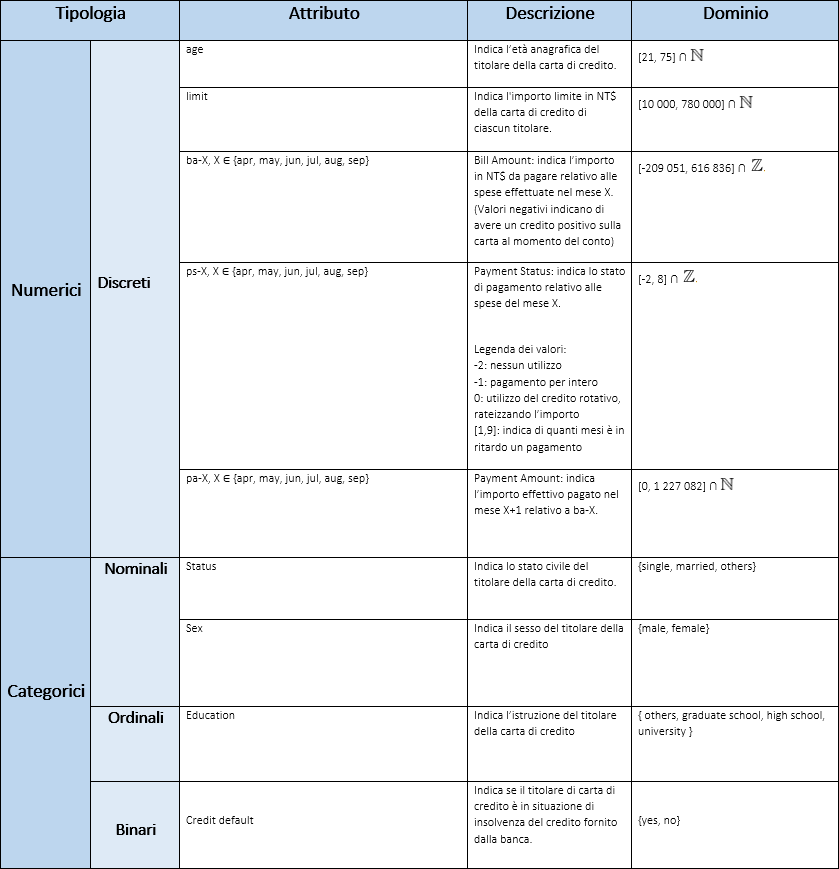
\includegraphics[width=13cm]{img/tabella1-attributi.png}
	\caption[LOF entry]{Attributi del dataset}
	\label{tab1attributi}
\end{table} 

\section{Analisi della qualità dei dati}
È stata analizzata la qualità dei dati all’interno del dataset fornito secondo i seguenti parametri:

\paragraph{Accuratezza sintattica}\mbox{}\\
È stata verificata la correttezza delle stringhe nei valori di attributi categorici \texttt{sex}, \texttt{education}, \texttt{status} e \texttt{credit\_default}. 
Sono stati analizzati i valori degli attributi numerici \texttt{limit}, \texttt{ps$-$\textit{X}}, \texttt{ba$-$\textit{X}} e \texttt{pa$-$\textit{X}} $(\texttt{\textit{X}} \in \{\texttt{\textit{apr,may,jun}}$,\\$\texttt{\textit{jul,aug,sep}}\})$ verificando che corrispondessero a valori presenti nel dominio fornito nei metadati del dataset. I dati forniti non presentavano errori a livello sintattico.
\mbox{}\\
\mbox{}\\
\paragraph{Accuratezza Semantica}\mbox{}\\
Dal punto di vista semantico sono stati analizzati nello specifico gli attributi \texttt{pa$-$\textit{X}}, \texttt{ba$-$\textit{X}} e \texttt{ps$-$\textit{X}}.
L’attributo \texttt{Payment Amount} è stato confrontato con l’attributo \texttt{Bill Amount} e \texttt{Payment Status} per verificare a quale importo di pagamento si riferisse il valore indicato \texttt{pa$-$\textit{X}}, ovvero se \texttt{pa$-$apr}, per esempio, indicasse un pagamento effettuato ad Aprile $($quindi relativo al conto di Marzo$)$ o un pagamento del conto di Aprile $($indicato da \texttt{ba$-$apr}$)$ e quindi effettuato a Maggio. Attraverso tale valutazione si è concluso che il valore  \texttt{pa$-$\textit{X}} indica il pagamento della cifra indicata dal \texttt{Bill Amount} del mese precedente. Questo corrisponde alla realtà poichè utilizzando una carta di credito, il pagamento effettuato in un mese X è relativo all’ importo da pagare del mese precedente. Riprendendo l’esempio precedente, il pagamento relativo al conto di Aprile $($\texttt{ba$-$apr}$)$ è indicato da \texttt{pa$-$may}. 
Da sottolineare la presenza di valori negativi nell’attributo \texttt{ba$-$\textit{X}}, rappresentanti dal punto di vista semantico una situazione di credito e non di debito nei confronti della banca.
\\
\begin{figure}[H]
	\centering
	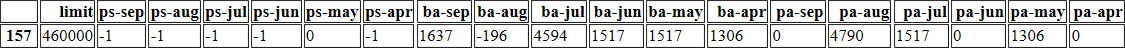
\includegraphics[width=\linewidth]{img/record-example.png}
	\caption[LOF entry]{un esempio di record che ha permesso facilmente di riconoscere il valore semantico degli attributi relativi alle transazioni monetarie. Si può notare grazie ai valori di \texttt{ps$-$\textit{X}}, come la cifra da pagare nel mese di Aprile, per esempio, sia equivalente alla cifra indicata nel pagamento di Maggio e lo stato di pagamento di aprile sia effettivamente -1, ovvero pagato completamente. Anche nei successivi mesi è possibile vedere un comportamento che corrisponde alla semantica degli attributi sopradescritta.}
	\label{record}
\end{figure}

Da sottolineare però che per verificare il corretto valore degli attributi  \texttt{pa$-$\textit{X}}, \texttt{ba$-$\textit{X}} e \texttt{ps$-$\textit{X}} sarebbe necessario conoscere tutta la cronologia delle transazioni di una specifica carta di credito così da poter calcolare attraverso semplici operazioni aritmetiche i valori effettivi di spese e pagamenti. Pertanto si è deciso di assumere come corretti i dati considerando inoltre che essendo informazioni raccolte da un istituto bancario non dovrebbero essere presenti dati monetari errati. 
\mbox{}\\
\mbox{}\\
\paragraph{Gestione di Outliers e Missing Values}\mbox{}\\
Per la ricerca di outliers è stato prodotto per ciascun attributo il relativo Boxplot, ma per la natura degli attributi del dataset, i valori rappresentati come outliers nel boxplot, non sono considerabili errati. Infatti per gli attributi numerici che rappresentano somme di denaro (\texttt{pa$-$\textit{X}}, \texttt{ba$-$\textit{X}} e \texttt{limit}), sarebbe scorretto considerare outlier, per esempio, una singola somma di denaro elevata poichè seppur sia un valore isolato, è un valore non errato ma concreto di uno specifico titolare di carta di credito in base a diversi fattori come il reddito. lo stesso ragionamento vale per gli attributi \texttt{age} e  \texttt{ps$-$\textit{X}}, poichè valori di età anagrafica o stati di pagamento che si discostano molto dall'andamento medio dei dati non possono considerarsi valori da eliminare.\\
L’utilizzo dei boxplot ha sollevato una problematica più facilmente osservabile del dataset, ovvero la presenza dei Missing Values:
\newpage
\textit{\textbf{attributi numerici}}: 
 nessun attributo numerico relativo al plafond $($\texttt{limit}$)$, allo stato del pagamento $($\texttt{ps$-$\textit{X}}$)$ o alle transazioni della carta $($\texttt{pa$-$\textit{X}}, \texttt{ba$-$\textit{X}}$)$ presentano missing values. Questi ultimi, presentano valori negativi o il valore 0, 
\begin{wrapfigure}{r}{9cm}
\centering
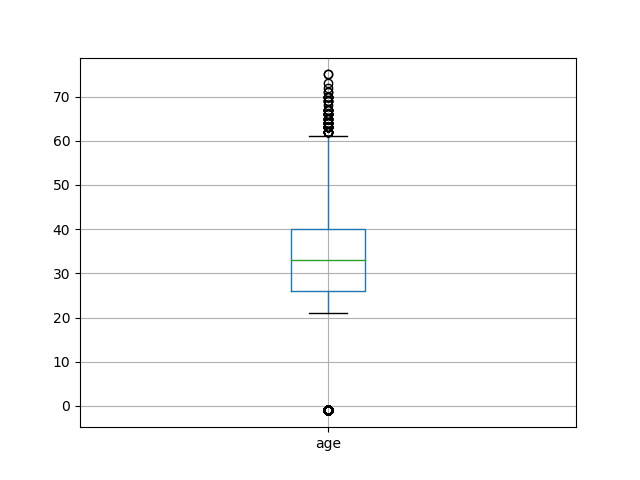
\includegraphics[width=8cm]{img/age-boxplot.png}
\caption{Boxplot del'attributo age}
\end{wrapfigure}
contenuti nel dominio di tali attributi. Per verificare aritmeticamente se i valori negativi o lo zero siano missing values, dovrebbe essere nota la cronologia completa delle transazioni relative a una carta ma avendo solamente dati relativi a un intervallo di tempo (Aprile 2005$-$Settembre 2005), non è stato possibile verificare se specifici valori nascondessero Missing Values.
Un attributo numerico che presenta un effettivo outliers è l’attributo \texttt{age}, infatti all’interno del dataset sono presenti per tale attributo molteplici valori -1, valore non coerente con un attributo che indichi l’età anagrafica. È facilmente intuibili come tale valore indichi un valore mancante. Pertanto, tale valore è stato sostituito con la media dell’età anagrafica dei record del dataset, ovviamente non tenendo conto dei valori -1. La media corrisponde a 35.4 che (per coerenza con il tipo di dato intero dell’età) è stata arrotondata a 35 e settata in sostituzione del valore -1.\\\\
\textit{\textbf{attributi categorici}}: ad eccezione di \texttt{credit\_default}, in ciascuno degli altri attributi categorici sono presenti missing values (nan), sostituiti dalla moda dell’attributo:
\begin{itemize}
\item \textbf{\texttt{sex}}: moda "female"
\item \textbf{\texttt{education}}: moda "university"
\item \textbf{\texttt{status}}: moda "single"
\end{itemize}

\section{Normalizzazione delle variabili}
Gli attributi \texttt{limit}, \texttt{ba$-$\textit{X}} e \texttt{pa$-$\textit{X}} rappresentando somme di denaro e pagamenti, hanno un ampio range di valori con massimo e minimo molto discostanti. Per utilizzare e visualizzare al meglio questi 3 attributi è stata utilizzata una normalizzazione \textbf{min-max}, trasformando il loro dominio in un range di valori continui [0,1].

\section{Distribuzione delle variabili e analisi statistiche}
\textbf{Attributi Numerici}\\
Per la visualizzazione della distribuzione di attributi numerici sono stati utilizzati degli istogrammi con curva gaussiana. Per gli attributi \texttt{limit},  \texttt{ba$-$\textit{X}}, \texttt{pa$-$\textit{X}}” e \texttt{age} si è scelto un numero di bins ottimale pari a 15 utilizzando la regola di Sturge, mentre per gli attributi  \texttt{ps$-$\textit{X}}, avendo un ristretto range di valori [-2, 8] si è utilizzato un numero di bins pari al numero di valori dell’attributo.

\begin{figure}[!htb]
\minipage{0.30\textwidth}
  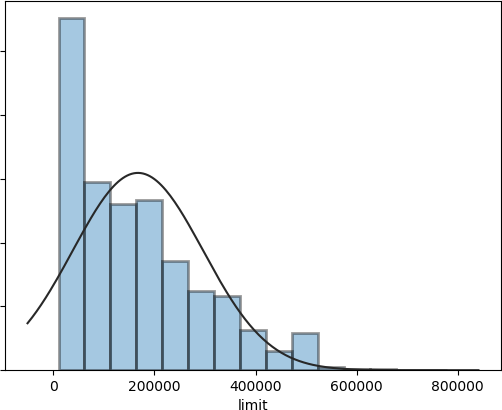
\includegraphics[width=\linewidth]{img/limit-distribution.png}
  \caption{Distribuzione attributo \texttt{limit}}\label{limit-dist}
\endminipage\hfill
\minipage{0.30\textwidth}
  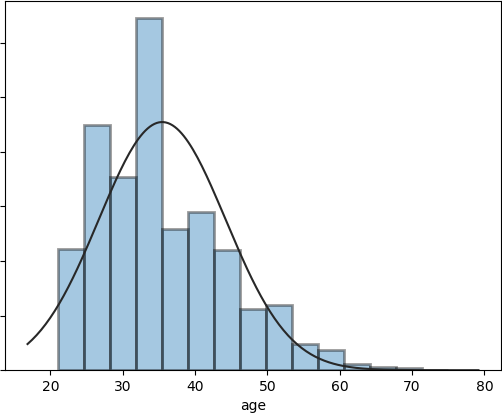
\includegraphics[width=\linewidth]{img/age-distribution.png}
 \caption{Distribuzione attributo \texttt{age}}\label{age-dist}
\endminipage\hfill
\minipage{0.35\textwidth}
  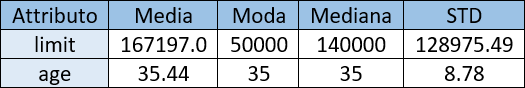
\includegraphics[width=\linewidth]{img/limit-age-stat.png}
\captionsetup{labelformat=empty}
\caption{Tabella 1.2: valori statistici \texttt{limit e age}}
	\label{limit-age-stat}
\endminipage
\end{figure}

Attraverso l'istogramma dell'attributo \texttt{limit} $($ Figura~\ref{limit-dist}$)$ è possibile vedere come vi sia una distribuzione inversamente proporzionale alla somma di denaro che la banca mette a disposizione del titolare di carta di credito. Un comportamento dei dati che rispecchia la realtà, evidenziando come le persone più facoltose e con limiti di carta di credito più alte siano anche le meno numerose. L'attributo \texttt{age} segue una distribuzione normale, infatti si può notare in Figura~\ref{age-dist} come il picco dell'istogramma coincida con la curva distribuzione, esattamente sul valore 35.

\begin{figure}[!htb]
\minipage{0.62\textwidth}
  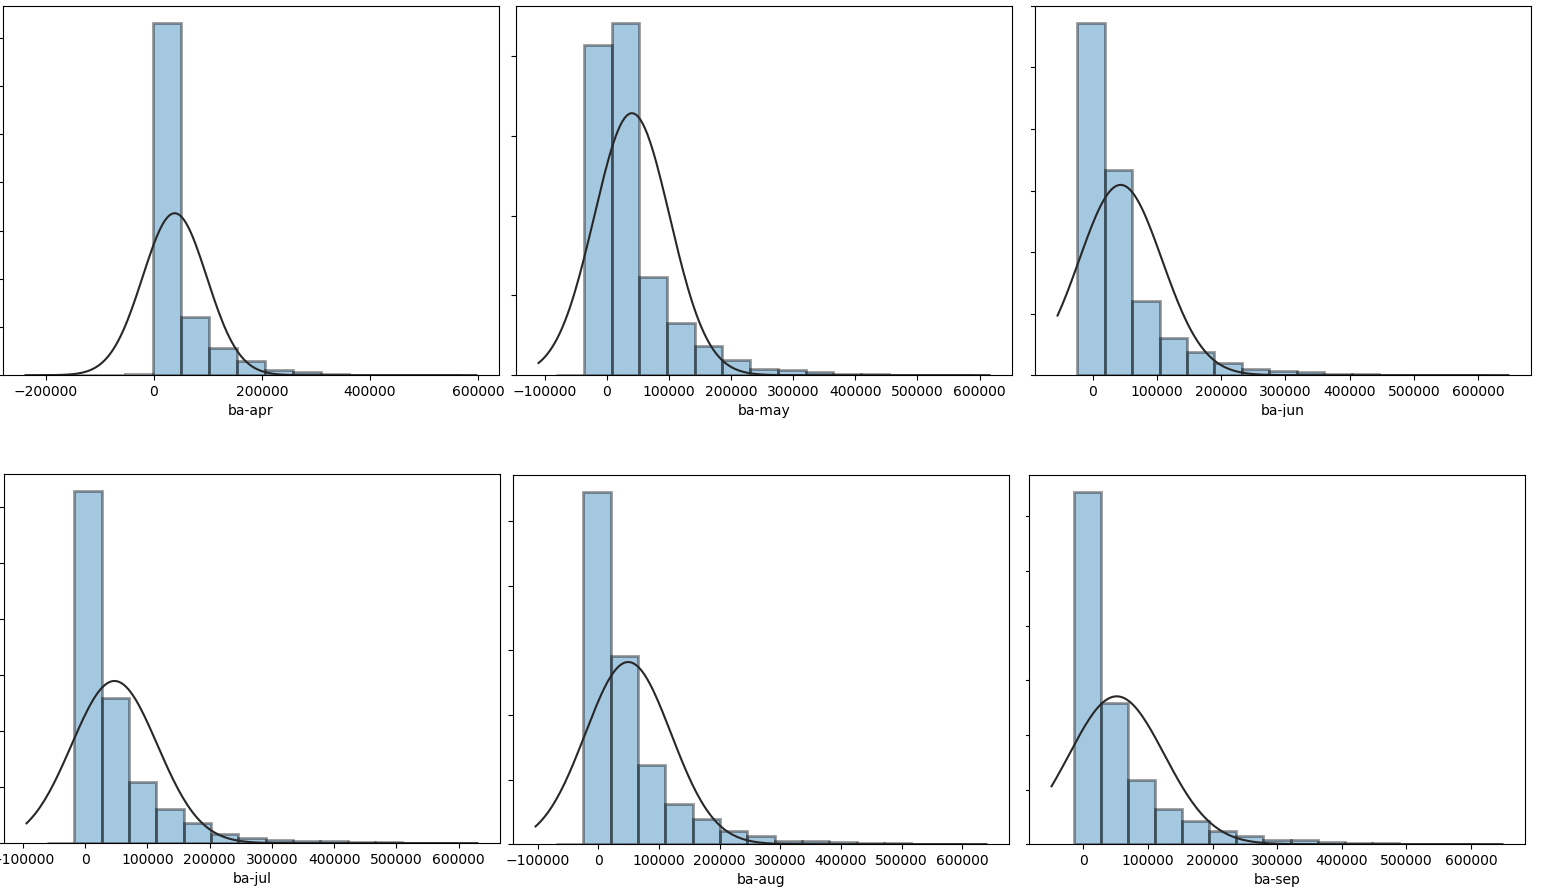
\includegraphics[width=\linewidth]{img/ba-distribution.png}
  \caption{Distribuzione attributo \texttt{ba-X}}\label{ba-dist}
\endminipage\hfill
\minipage{0.34\textwidth}
  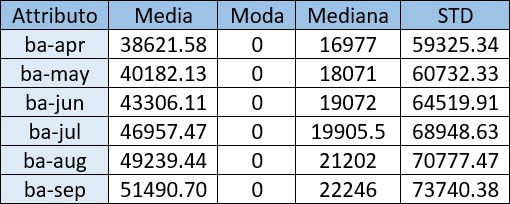
\includegraphics[width=\linewidth]{img/ba-stat.png}
\captionsetup{labelformat=empty}
\caption{Tabella 1.3: valori statistici \texttt{ba$-$\textit{X}}}
\label{ba-stat}
\endminipage\hfill
\end{figure}

\begin{figure}[!htb]
\minipage{0.62\textwidth}
  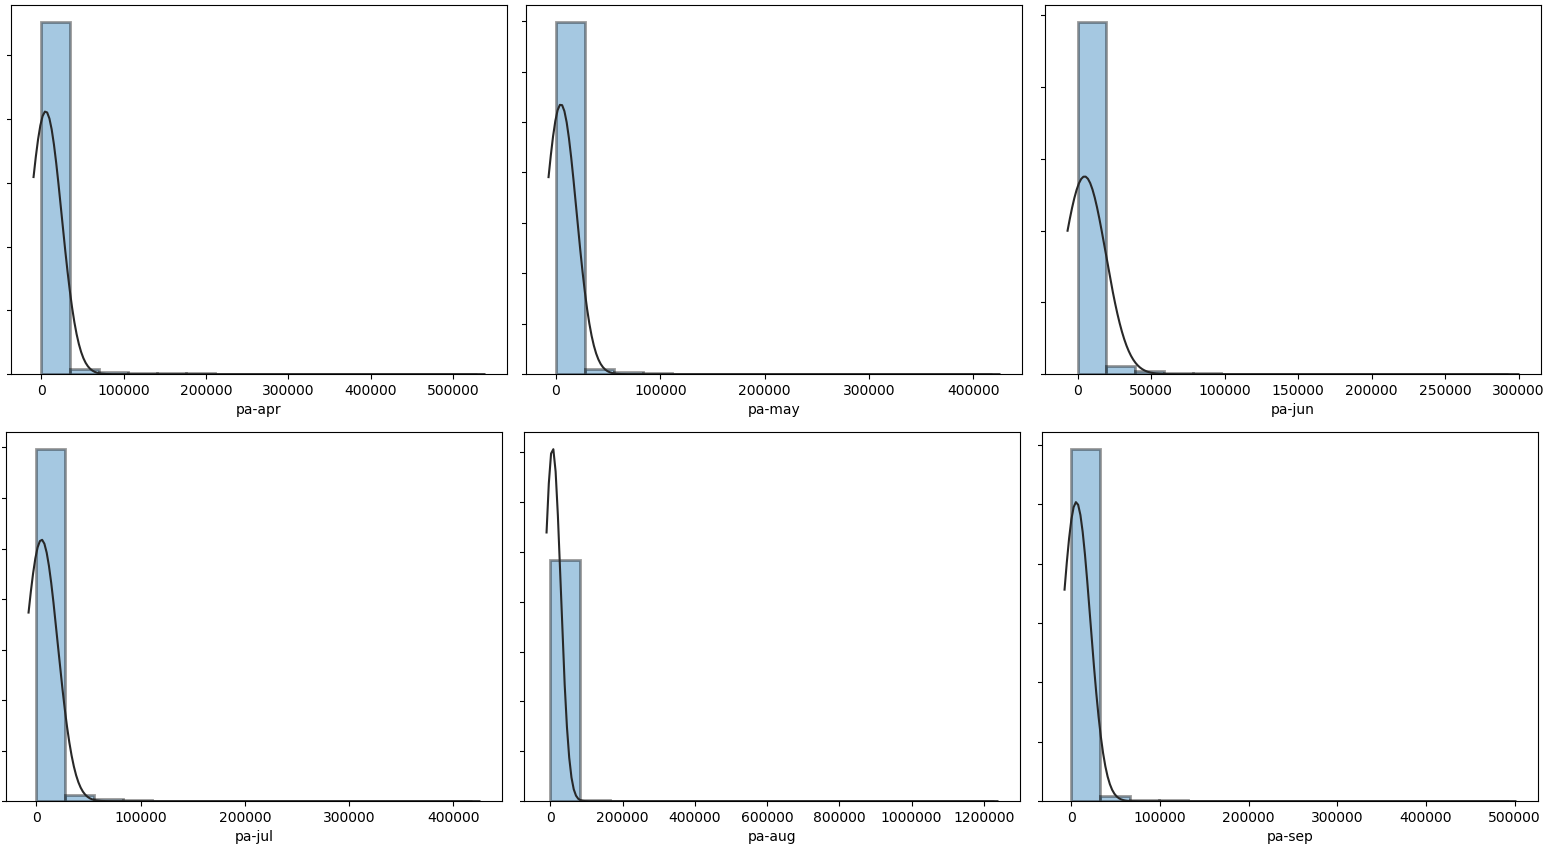
\includegraphics[width=\linewidth]{img/pa-distribution.png}
  \caption{Distribuzione attributo \texttt{pa-X}}\label{pa-dist}
\endminipage\hfill
\minipage{0.34\textwidth}
  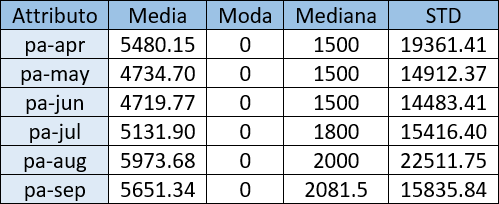
\includegraphics[width=\linewidth]{img/pa-stat.png}
\captionsetup{labelformat=empty}
\caption{Tabella 1.4: valori statistici \texttt{pa$-$\textit{X}}}
\label{pa-stat}
\endminipage\hfill
\end{figure}
\mbox{}\\
Per i gli attributi relativi al \texttt{Bill Amount} e al \texttt{Payment Amount} è possibile osservare picchi elevati per valori bassi. E' osservabile come il valore più ricorrente in entrambi i casi sia 0, ovvero che la maggior parte dei titolari di carta ogni mese non abbiano da pagare nessuna somma di denaro. Si può come nonostante siano presenti valori medi di \texttt{Bill Amount} piuttosto alti, per ogni mese il Payment Amount ha un valore medio di circa 5000. Osservando gli istogrammi in figura 1.10 e la Tabella 1.5 relativi ai Payment Status, si può giustificare la differenza di valori medi degli attributi \texttt{Bill Amount} e \texttt{Payment Amount} da un alto numero di titolari di carta che ricorrono al metodo di pagamento \textbf{revolving credit}, rappresentato dal valore 0 degli attributi \texttt{Payment Status}, valore più ricorrente.
Inoltre è da sottolineare come gli attributi \texttt{Payment Status} seguano a grandi linee una distribuzione normale, con picco sul valore 0.
\begin{figure}[!htb]
\minipage{0.62\textwidth}
  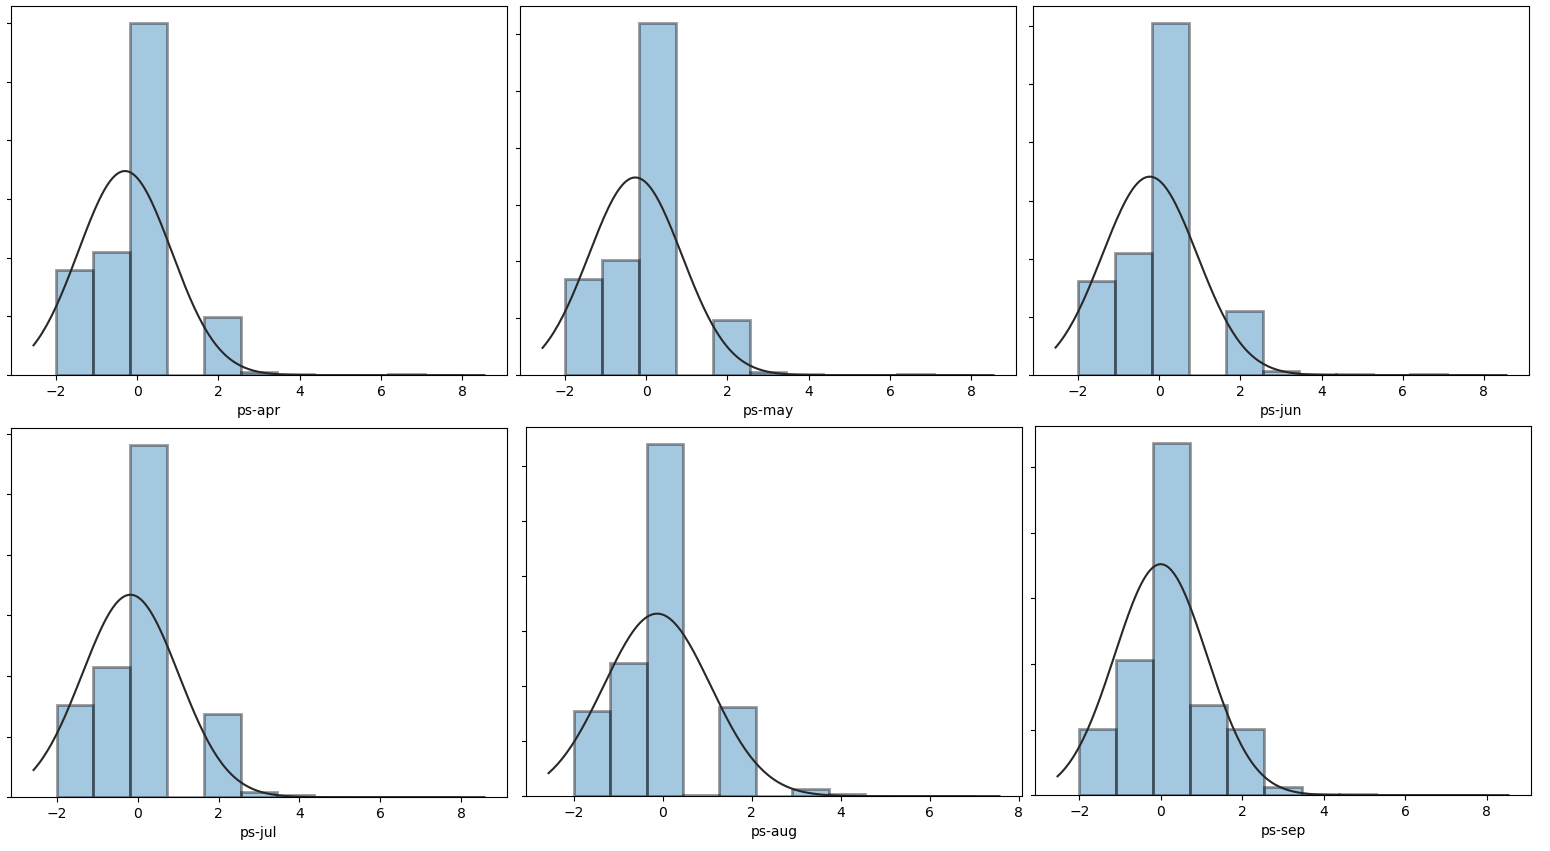
\includegraphics[width=\linewidth]{img/ps-distribution.png}
  \caption{Distribuzione attributo \texttt{ps-X}}\label{ps-dist}
\endminipage\hfill
\minipage{0.34\textwidth}
  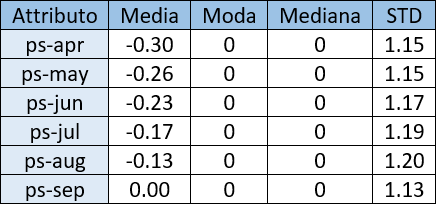
\includegraphics[width=\linewidth]{img/ps-stat.png}
\captionsetup{labelformat=empty}
\caption{Tabella 1.5: valori statistici \texttt{ps$-$\textit{X}}}
\label{ps-stat}
\endminipage\hfill
\end{figure}
\\
\textbf{Attributi Categorici}\\
\begin{figure}[!htb]
\minipage{0.48\textwidth}
  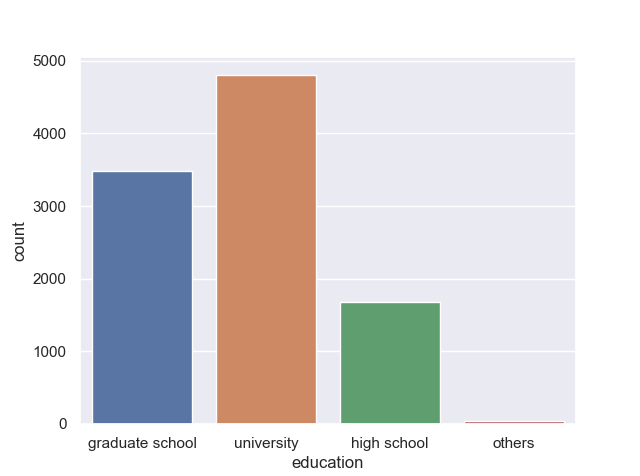
\includegraphics[width=\linewidth]{img/education-hist.png}
  \caption{Istogramma attributo \texttt{education}}\label{edu-dist}
\endminipage\hfill
\minipage{0.48\textwidth}
  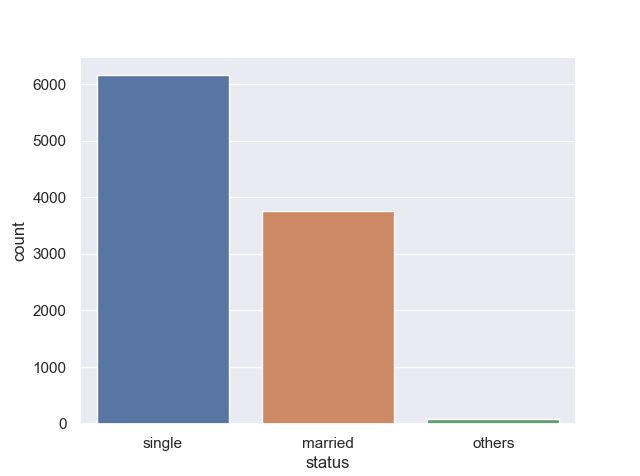
\includegraphics[width=\linewidth]{img/status-hist.png}
  \caption{Istogramma attributo \texttt{status}}\label{status-dist}
\endminipage\hfill
\end{figure}
\mbox{}\\\mbox{}\\

Per gli attributi categorici \texttt{education} e \texttt{status} sono stati generati gli istogrammi riportati in figura 1.12 e 1.13, mentre per gli attributi binari \texttt{sex} e \texttt{credit\_default} si è preferito l'utilizzo di grafici a torta.

\begin{figure}[!htb]
\minipage{0.48\textwidth}
  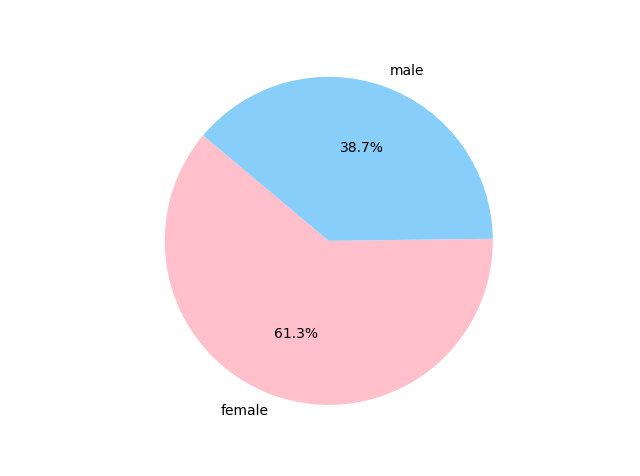
\includegraphics[width=\linewidth]{img/sex-dist.png}
  \caption{Istogramma attributo \texttt{sex}}\label{sex-dist}
\endminipage\hfill
\minipage{0.48\textwidth}
  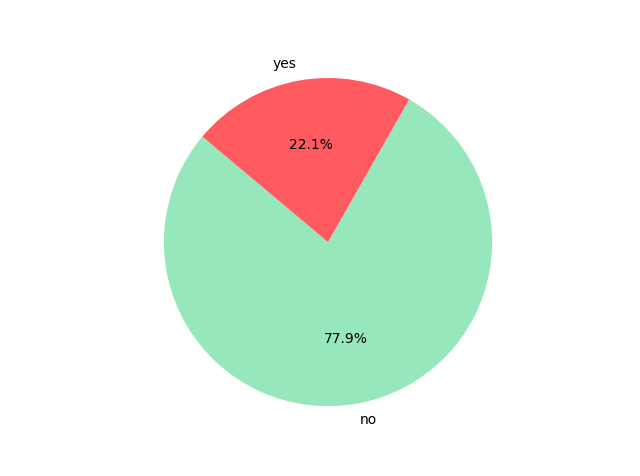
\includegraphics[width=\linewidth]{img/default-dist.png}
  \caption{Istogramma attributo \texttt{credit\_default}}\label{default-dist}
\endminipage\hfill
\end{figure}
\newpage
\section{Correlazione tra variabili}
\begin{figure}[!htb]
\centering
  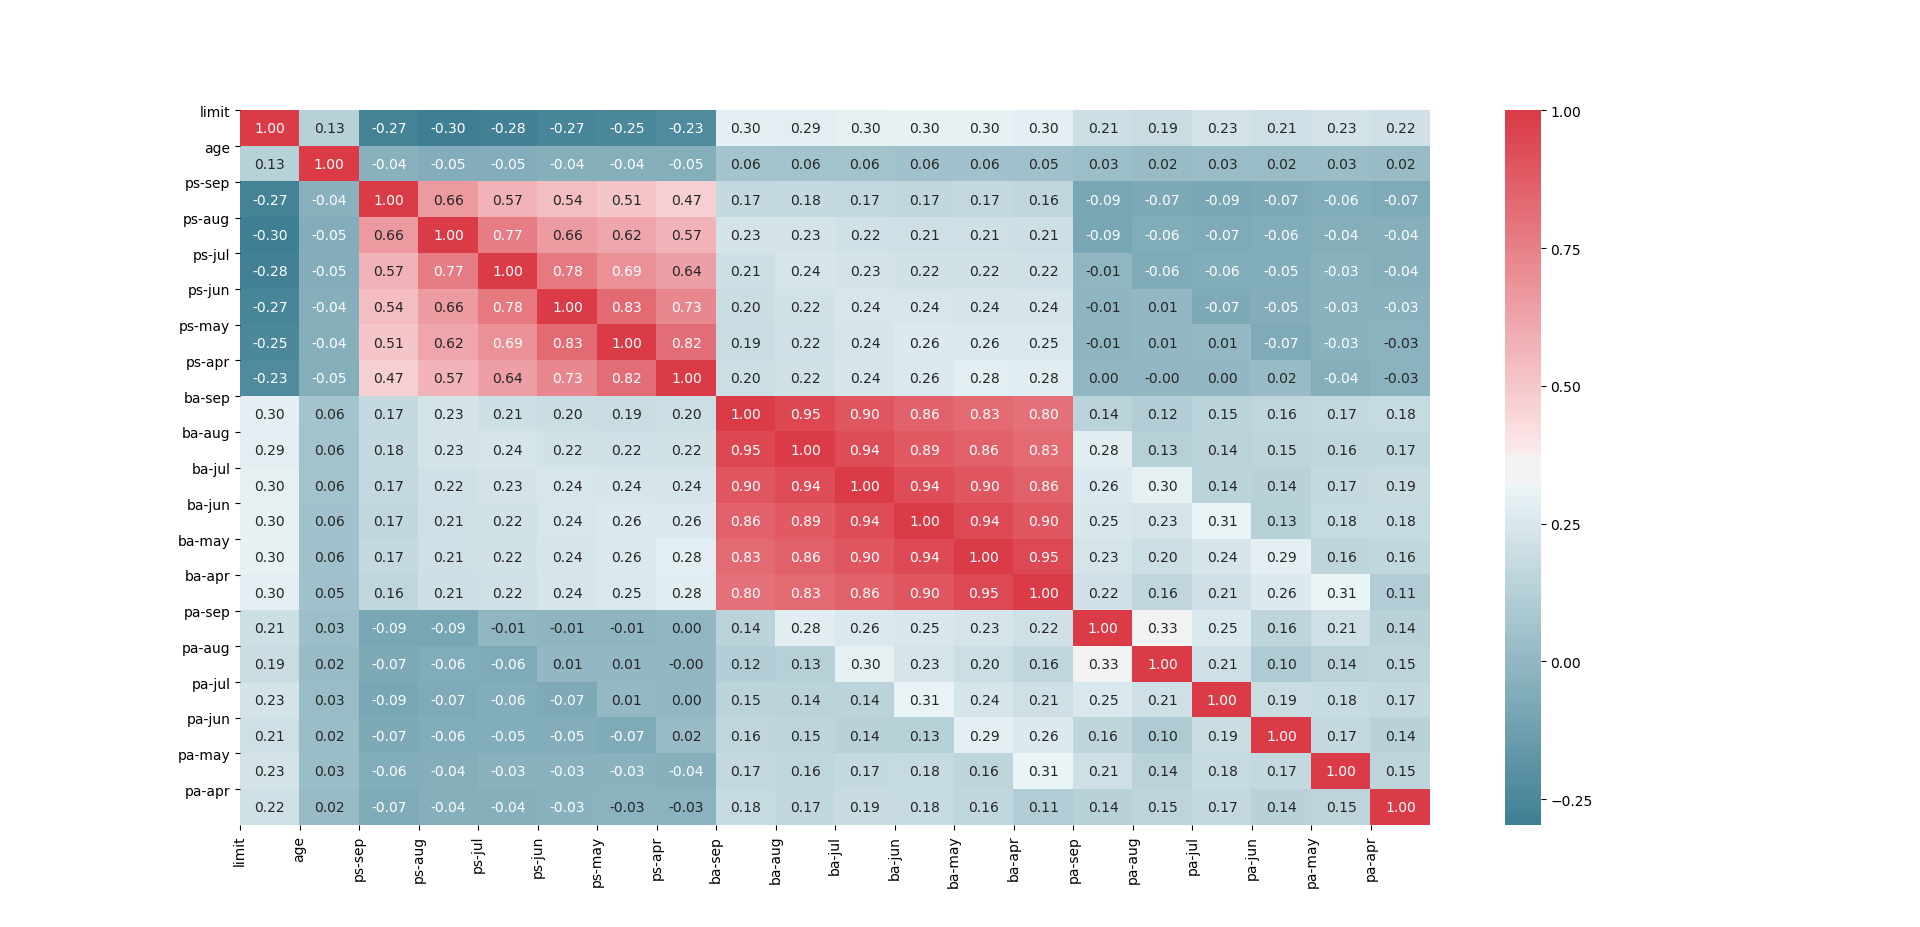
\includegraphics[width=\linewidth]{img/heatmap.png}
  \caption{Heatmap delle correlazioni tra attributi}\label{heatmap}
\end{figure}

Scrivere baggianate sulla correlazione


